\documentclass[12pt]{article}

\usepackage{amsmath}
\usepackage{amssymb}
\usepackage{geometry}
\usepackage{graphicx}
\usepackage{hyperref}

\geometry{letterpaper,tmargin=1in,bmargin=1in,lmargin=1in,rmargin=1in}

\hypersetup{
colorlinks, linkcolor=blue,
}


\begin{document}

\title{Analog IC Design: Project - Part 1}
\date{Spring 2018}
\maketitle
\tableofcontents

\newpage
\section{Objective}

In part 1 of this project I will be designing a Operational-Amplifier from scratch. This will be done by following a step by step incremental process. This allows for the understanding of each component of the circuit before moving forward to more complicated steps.


\section{Custom MOSFETS}
\label{sec:desigan_and_analysis}

In the following design we will be given both a NMOS and PMOS transistors. The characteristics of these MOSFETs are as follows.

\begin{itemize}
	\item NMOS \newline \newline
	.SUBCKT enmos001 1 2 3 \newline
	M 1 2 3 3 enmos001\newline
	.MODEL enmos001 NMOS (KP = 500E-6 VTO = 1 LAMBDA = 0.02 W=2u L=1u)\newline
	.ENDS enmos001
\newline
	\item PMOS \newline \newline
	.SUBCKT enmos002 1 2 3 \newline
	M 1 2 3 3 enmos002\newline
	.MODEL enmos002 PMOS (KP = 500E-6 VTO = 1 LAMBDA = 0.02 W=2u L=1u)\newline
	.ENDS enmos002
\newline
	
\end{itemize}

Using Multisim's component wizard we can import this settings and create custom MOSFETs for use in our simulation.

\subsection{Problems Encountered}
In the following section when creating a CS amplifier with a current source load, the above MOSFETs where causing numerous problems in Multisim 13. Gain was non-existent and the voltage at the Gate and Drain were well above 500 GigaVolts for some unknown reason. Transferring the circuit into Multisim 14.1 solved this problem.

\section{Common-Source Amplifier with Ideal Current Source}


The following circuit is using both a ideal current source, high resistor, and infinite capacitance; all are things that must be replaced before the final circuit. But it will serve as a step in the right direction.


\begin{figure}[t]
	\label{fig:amp}
	\caption{Given CS Amplifier}
	\centering
	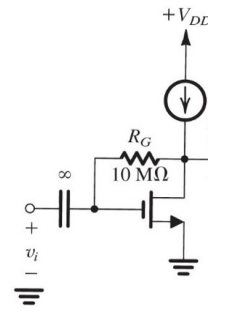
\includegraphics[width=.3\textwidth]{csamplifier}
\end{figure}



\subsection{Region of Operation}
The Common-Source Amplifier will be operating in the Saturation Region, this is because $V_g$ is connect directly to $V_d$. This results in $V_{gs}$ being greater than $V_t$.

$$V_{DS} = V_{GS}$$
$$V_{DS} > V_{VOV}$$
$$V_{DS} > V_{GS} - V_t$$

This when used with the IV-Characteristics graph show the the amplifier will be operating in saturation.

\subsection{Small-Signal Model}
By modeling our CS Amplifier with the Small-Signal Model we can derive the relationship for gain.


\begin{figure}[h]
	\label{fig:amp}
	\caption{Small-Signal Model}
	\centering
	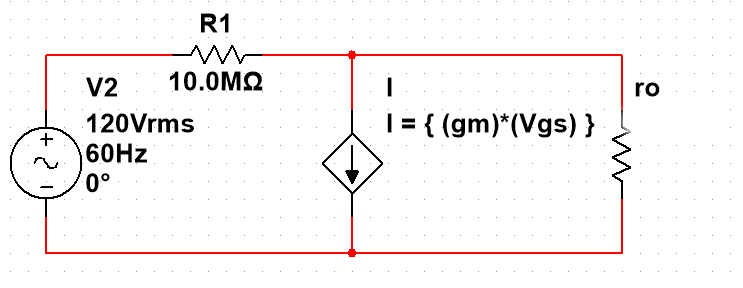
\includegraphics[width=.65\textwidth]{smallsignal}
\end{figure}

With the small-signal model we can see that the resistor $R_1$ is so large that  $V_{GS}$ will be the same as $V_2$ which is our $v_o$. This means that the current from current source $I$ will be drawn into resistor $r_o$ then back two the current source. With this we can see that,

$$V_o = -g_m r_o V_{GS}$$
$$\frac{v_o}{V_{gs}}  = -g_m r_o$$
$$G = -g_m r_o $$
Knowing that the following is true
$$g_m = \sqrt{2K_n I_d}$$
$$r_o = \frac{1}{\lambda I_d}$$

 We can now arrive at the solution
$$G = -\frac{1}{\lambda} \sqrt{\frac{2 K_n}{I_d}}$$


\subsection{Manipulating $I_d$ for a gain of 100}

With the equation derived in the previous section we can now use our MOSFET characteristics to find a value for current $I$ that will result in a gain of 100.

$$G = -\frac{1}{\lambda} \sqrt{\frac{2 K_n}{I_d}}$$

Replacing $K_n$ with $K'_n$ we can derive the equation farther.


$$G = -\frac{1}{\lambda} \sqrt{\frac{2 K'_n \frac{W}{L}}{I_d}}$$

Now we can enter our constants and solve for $I_d$

$$100 = -\frac{1}{.02} \sqrt{\frac{2*500*10^6 \frac{2}{1}}{I_d}}$$

$$100 = -50 \sqrt{\frac{.002}{I_d}}$$

$$-2 = \sqrt{\frac{.002}{I_d}}$$

$$4 = \frac{.002}{I_d}$$

$$I_d = .5mA$$

So in order to obtain a gain of 100 in our CS Amplifier we need a $I_d$ value of $.5mA$


\subsection{Simulation Verification}

By simulating Figure 1 in Multisim with the calculated value $I$ we can verify the accuracy of our previous calculation

\begin{figure}[h]
	\label{fig:amp}
	\caption{Gain Verification}
	\centering
	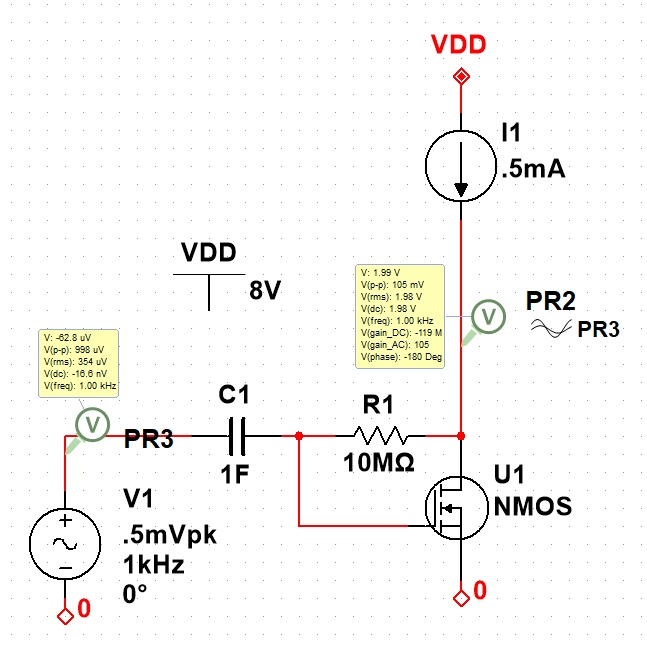
\includegraphics[width=.5\textwidth]{cssimulation}
\end{figure}

The figure above shows that out calculations where correct. With a $I_d$ value of $.5mA$ we are arriving at a gain of about $100$

By also manually measuring the value of $V_{DS}$ and $V_{GS}$ we can show that the amplifier is indeed operating in the saturation region.

\begin{figure}[h]
	\label{fig:amp}
	\caption{$V_{DS}$ and $V_{GS}$}
	\centering
	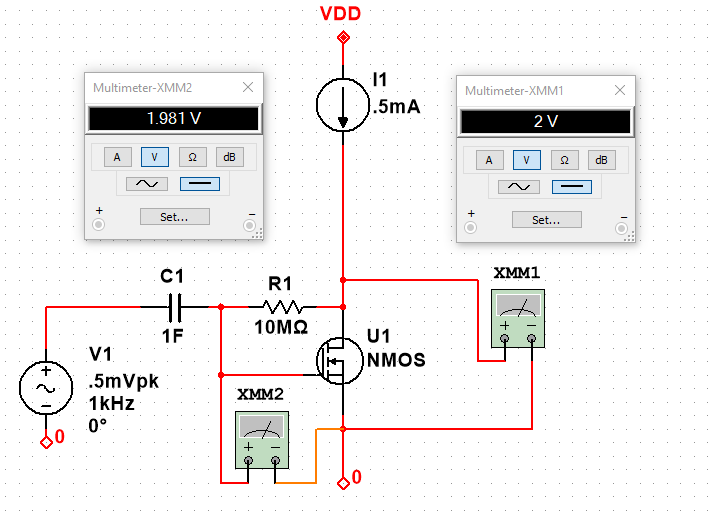
\includegraphics[width=.4\textwidth]{vgs}
\end{figure}

$$V_{DS} > V_{GS}- V_t$$
$$2V > .981V$$

The measurements prove our previous assumptions

\section{Common-Source Amplifier with Current Source load}
So now that we can model the common-source amplifier with an ideal source we can progress by replacing the ideal source with a circuit that will act the same. The following next circuit will do that and eliminate the need for a large feedback resistor for biasing.

\begin{figure}[h]
	\label{fig:amp}
	\caption{Non-Ideal Circuit}
	\centering
	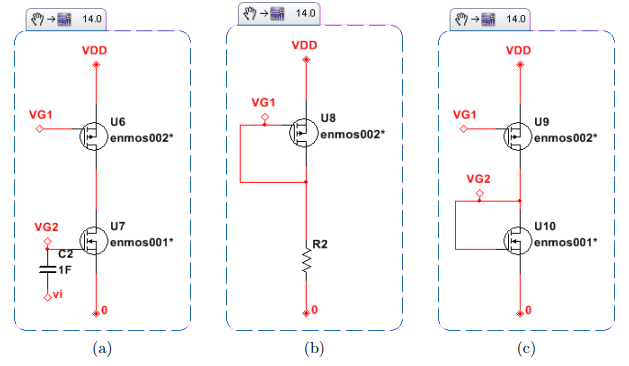
\includegraphics[width=.5\textwidth]{nonideal}
\end{figure}

\subsection{Calculating the new gain}

If we take the same $I_d$ that was calculated above and apply it to our circuit now, what happens to our gain? Using the small signal model we can once again go ahead and find a suitable equation.

\begin{figure}[h]
	\label{fig:amp}
	\caption{Small-Signal Analysis}
	\centering
	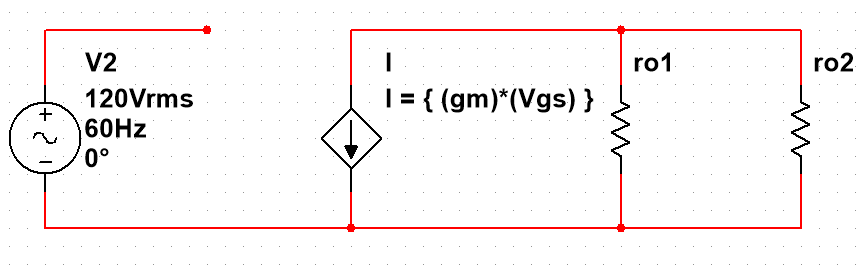
\includegraphics[width=.5\textwidth]{smallsignal2}
\end{figure}

From the above model we can see that the PMOS transistor is in the place of our ideal current source. But when this happens it causes its $r_{o2}$ value to now be in parallel with our $r_{o1}$ NMOS resistor.

Using our knowledge from section 3.1.2 we can see that our new gain equation will be,

$$G = \frac{V_o}{V_i} = -g_{m1} (r_{o1}||(r_{o2}))$$
Simplified knowing that $r_{o1} = r_{o2}$
$$G = -\frac{1}{2}g_{m1}r_o$$
This means that the gain of this circuit will be half that of the previous circuit in figure 1. So the gain with $I_d = .5mA$ will be $50$

\subsection{Finding the Resistor Value}

Now that we understand the gain ratio we will be achieving, we must calculate $R_2$ in the given circuit such that $I_d$ is equal to the ideal-source amplifier. Because in circuit B $V_G = V_D$, we can use the PMOS current equation. With that and Ohms law we can solve for $R_2$

$$I_d = \frac{1}{2} K_p (V_{S1} - V_{G1}- |V_t| )^2$$
$$.5mA = \frac{1}{2} .001 (8-V_{G1} - 1)^2   $$
$$V_d = V_{G} = 6V$$
$$R_2 = \frac{V_d}{I_d} = 12k\Omega$$


\subsection{Simulation Verification}
By simulating in multisim we can ensure that all assumptions and calculation up until this point are correct.
\begin{figure}[h]
	\label{fig:amp}
	\caption{Amplifier Simulation}
	\centering
	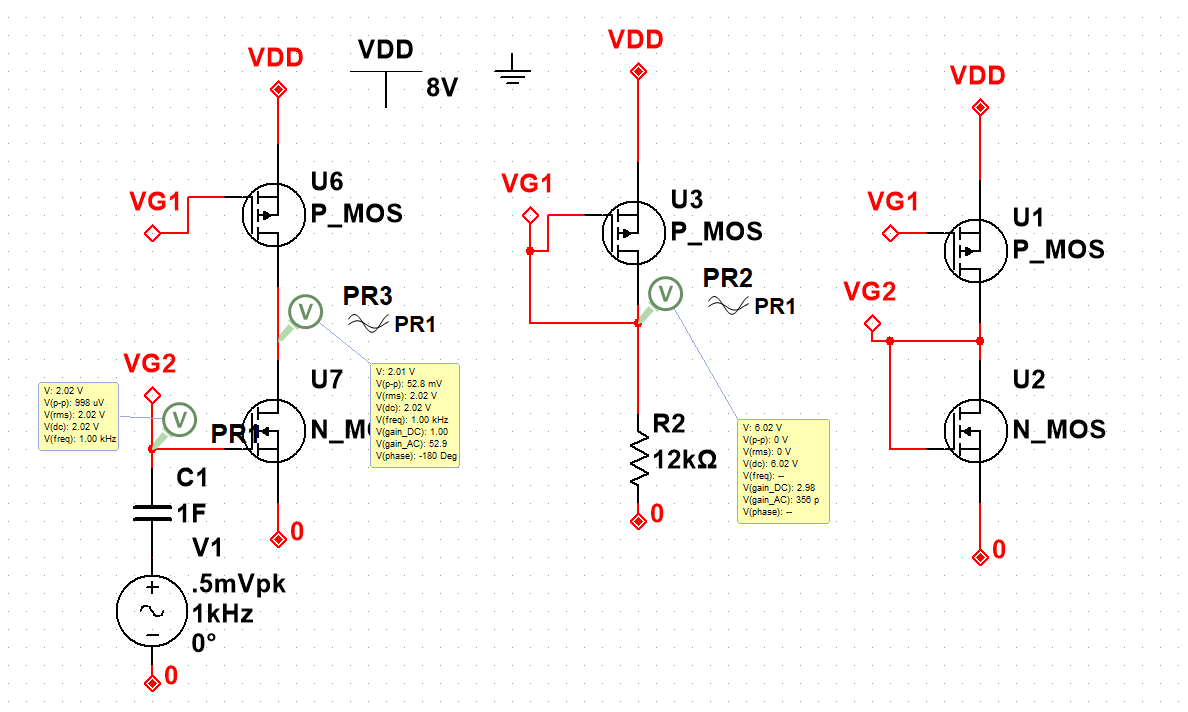
\includegraphics[width=1\textwidth]{simulation2}
\end{figure}
In figure 7 you can see that Probe 2 in reference to Probe 1 is seeing a gain of about $50$ which is correct from our calculation in section 4.1.

\section{Differential Amplifier}
From the understanding gathered in the above sections we can now create a full fledge differential amplifier. The requirements are as follows.

\begin{enumerate}
	\item Two power supplies $V_{DD}$ and $V_{SS}$.	
	\item One reference resistor $R_{REF}$ (which will be outside your IC
	\item Any number of n-channel and p-channel MOSFETS. You may edit the models for each
	MOSFET according to you design
\end{enumerate}

Also to obtain a the desired currents and biasing voltages, current steering and mirrors are recommended.


\subsection{Circuit Design}
The design that I arrived is at follows. The sections are colored to show what portion of the circuit does what.


\begin{figure}[h]
	\label{fig:amp}
	\caption{Circuit Explanation}
	\centering
	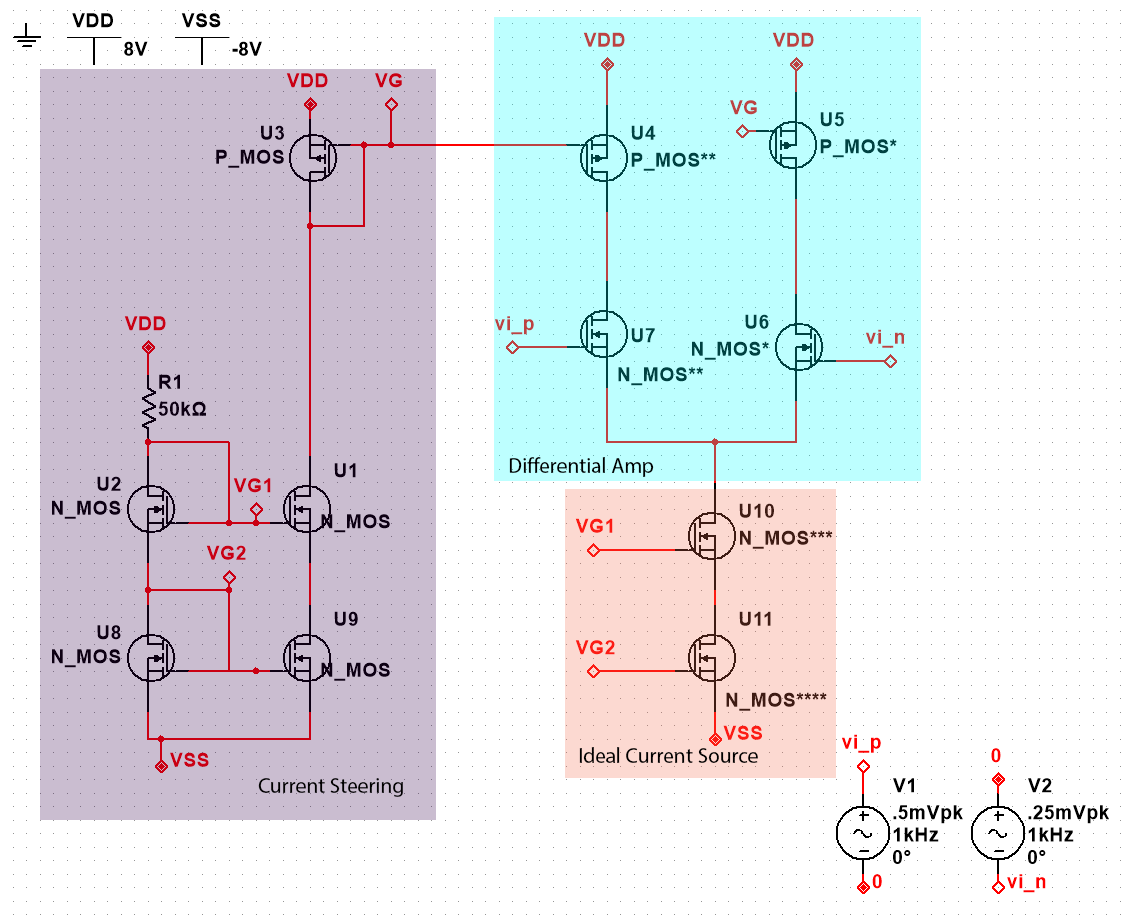
\includegraphics[width=.8\textwidth]{photoshop}
\end{figure}

The value of the resistor was calculated using section 4.2. By Solving for $V_{GS}$ while setting current to $250\mu A$ and still using the assumption that $V_{DS} = V_{GS}$.This resistor acts as a voltage divider to give the exact amount of voltage needed to the current steering circuit. Also by simplifying the math by using a width of $2\mu m$ we can find what we need.\

$$G = \frac{1}{2} g_m r_o = \frac{1}{2} (\frac{1}{\lambda I_D}) \sqrt{2K_n I_D}$$
$$I_D = .25mA$$
$$250\mu = \frac{1}{2}  K_n (V_{g2} - V_s - V_{tn} )^2(1 + \lambda V_{g2} -\lambda V_s)    $$

$$V_{g2} = -6.3V$$

$$250\mu = \frac{1}{2}  K_n (V_{g3} - V_s - V_{tn} )^2(1 + \lambda V_{g3} -\lambda V_s)    $$

$$V_{g3} = -4.8V$$

$$R_{ref} = \frac{V_{g3} }{I_d}\eqsim 50k\Omega$$



\subsection{Analysis}
The analysis of the designed circuit shows that a gain of $100$ is being obtained. This is at Probe 1 in reference to Probe 4.

\begin{figure}[h]
	\label{fig:amp}
	\caption{Final Circuit Analysis}
	\centering
	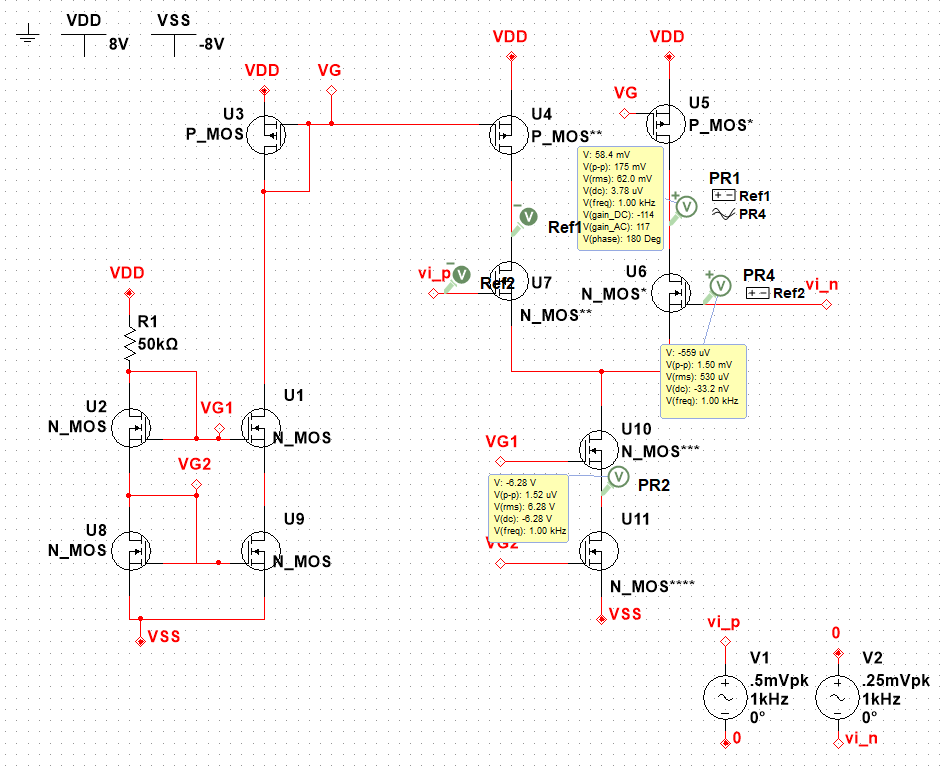
\includegraphics[width=1\textwidth]{finalamp}
\end{figure}



\section{Conclusion}
The project so far has been challenging but rewarding. In terms of progress so far, by chopping the assignment into pieces and individual circuits it made tackling the final circuit that much easier. The Differential amplifier using the given transistors does in fact work, which on its own is very satisfying. I look forward to continuing and completing the design.





\end{document}
